\documentclass[Eubank_pk_ethnic_sorting.tex]{subfiles}


\begin{document}

The focus of this paper is the rural, secular, primary school educational ecosystem of 112 randomly selected villages (\emph{mauzas}) in the Punjab districts of Attock, Faisalabad, and Rahim Yar Khan in Pakistan. These 112 villages were the subject of the Learning and Educational Attainment in Punjab Schools (LEAPS) panel survey. LEAPS villages were selected through probability proportional to population sampling (stratified at the district level) from the universe of all villages in these districts with at least one private school. The survey ran from to 2003-2007, and includes detailed surveys of households, students, teachers, and both government and private schools in these villages. In addition, some data used in this analysis comes from a listing census conducted in sample villages prior to the start of the LEAPS survey that include basic demographic information on all households, allowing for the computation of accurate village level statistics.

The LEAPS survey is organized around two panels of students -- one (initiated in 2003 with an initial population of 12,110 children) which followed students for four years, and one (initiated in 2005 with an initial population of 11,852 students) which followed students for two years. Each panel represents the universe of enrolled students in sample villages in Class 3 at the time of panel initiation in both government and private schools. Students and their teachers in both panels were administered annual exams in English, math, and Urdu by the LEAPS team, and these tests were subsequently standardized using Item Response Theory (IRT) methods.

\subsection{Caste in Punjab}\label{caste_in_punjab}

This paper focuses on how village-level caste politics influence the selection of students into private and government schools. Before directly examining this dynamic, however, some background on the nature of caste in Pakistan is warranted.

Caste -- known variously as \emph{biraderi}, \emph{zaat}, or \emph{qaam} -- is a central aspect of rural social identity in Pakistan, especially in Punjab. While \emph{biraderi} is a somewhat distinct concept from the idea of ``caste'' in India, ``it retains a very important feature of the [Indian subcaste] -- that of an inherent, inbuilt hierarchy that governs social interactions. Society is hierarchically ordered with the Syeds at the top, followed by the landowning castes, then by the service castes or kammis, and finally by the Musallis, who occupy the lowest rung of the social ladder. This ordering dictates much of the social life in a Punjabi village and is most profound in the notions of community cooperation, where solidarity is strongest within a biraderi.''\citep[p. 29]{Gazdar:2007vt}.

\emph{Biraderi} is correlated with wealth, land holdings, and education, but it is not synonymous with economic class. As a related report observes, ``while economic power is required to reinforce biraderi-based dominance, membership of a dominant biraderi can help mitigate some of the effects of being economically poor. As one respondent put it, `the poorest Jatt is still better off than the richest kammi.''' \citep[p. 13]{Gazdar:2007vt}

\subsection{Village Caste Composition}\label{context_village_composition}

While the centrality of caste politics is relatively universal across villages in Punjab, however, there is significant variation in village \emph{biraderi} composition. Figure~\ref{fracdensities} below shows the density plot of villages of different levels of caste fractionalization, measured as one minus a herfindahl index.\footnote{One minus the herfindahl index is a common measure of fractionalization equal to the probability that any two randomly selected individuals belong to the same group. Village fractionalization is computed using data from a village census conducted in 2002 to facilitate household sampling for the LEAPS survey which includes data on the \emph{biraderi} of all households in LEAPS villages.} As the figure shows, there is significant variation in the degree of fractionalization both within and across the three districts of the LEAPS survey.

\begin{figure}[htb]
	\begin{center}
	\caption{Village Caste Fragmentation by District}\label{fracdensities}
	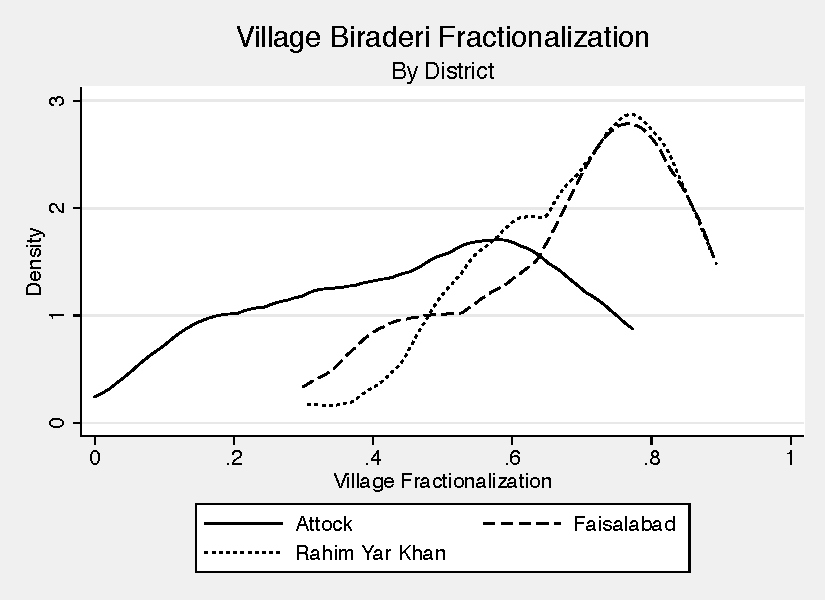
\includegraphics[scale=1.0]{../results/village_frac_by_district.pdf}
	\end{center}
\end{figure}

As shown in Table~\ref{villagebyfrac}, this variation in heterogeneity is not clearly related to village wealth, land inequality, or adult education. There is some relationship to village size, but on the whole fractionalization appears to be relatively independent of other village characteristics.

\begin{table}[htbp]\centering
\def\sym#1{\ifmmode^{#1}\else\(^{#1}\)\fi}
\caption{Village Characteristics and Fractionalization\label{villagebyfrac}}
\begin{tabular}{l*{6}{c}}
\toprule
                &\multicolumn{1}{c}{(1)}&\multicolumn{1}{c}{(2)}&\multicolumn{1}{c}{(3)}&\multicolumn{1}{c}{(4)}&\multicolumn{1}{c}{(5)}&\multicolumn{1}{c}{(6)}\\
                &\multicolumn{1}{c}{\specialcellc{Median\\Wealth}}&\multicolumn{1}{c}{\specialcellc{Adult\\Literacy}}&\multicolumn{1}{c}{\specialcellc{Land\\Gini}}&\multicolumn{1}{c}{\specialcellc{Enrollment\\Pct}}&\multicolumn{1}{c}{\specialcellc{Schools\\per HH}}&\multicolumn{1}{c}{Log Num HH}\\
\midrule
Fractionalization&   -314.1   &    -6.66   &     0.10   &    -14.1   &   0.0010   &     0.64*  \\
                &  (146.8)   &   (15.0)   &  (0.074)   &   (13.3)   & (0.0073)   &   (0.21)   \\
District FE     &      Yes   &      Yes   &      Yes   &      Yes   &      Yes   &      Yes   \\
\midrule
Observations    &      112   &      112   &      112   &      112   &      112   &      112   \\
\bottomrule
\multicolumn{7}{l}{\footnotesize Standard errors in parentheses}\\
\multicolumn{7}{l}{\footnotesize * \(p<0.10\), ** \(p<0.05\), *** \(p<0.01\)}\\
\multicolumn{7}{l}{\footnotesize Standard errors clustered by District.}\\
\end{tabular}
\end{table}



\end{document}
